% !TeX spellcheck = en_US
\section{Rolling Road GUI}

The Rolling Road GUI helps control and visualize the data coming from the Rolling Road. Furthermore it allows for saving and importing recorded datasets in the CSV-Fileformat, making it possible to further analyze in Excel or a equivalent program.

The application is developed in the .Net framework by Microsoft and the code itself is written in C\#.
To help create a GUI(Graphical User Interface) the WPF library which is a part of the .Net framework was used, it uses XAML to layout the different views.

\subsection{Design \& Considerations}

Initially the 3-layer architecture use for the back-end and MVVM was used as front-end architecture. But later in the development cycle, the 3-layer architecture was changed to the Onion Architecture to help manage the many source files.

\fxnote{enten forklar lidt mere om 3-layer og Onion architecture eller referer til noget i dokumentationen der kan forklare hvad det er. JS}

The Onion-Architecture heavily uses the repository pattern to abstract away from the data source.\fxnote{lyder fint men ved ikke hvad det betyder. JS} Making it easy to change the datasource to a database for example later in the process, so if the website user story was to be implemented it would require little or no change to the 'backend'.

The communication with the Rolling Road is using the SP4RR protocol over a UART serial connection. In this case a USB-UART converter built into the PSoC is used to supply the computer with a uart connection, so only a Micro usb cable is needed to connect the two.

\subsection{Implementation}

Since some kind of plotting needed to be implemented, the search for a library started, the application originally used the WPF Toolkit data visualization\cite{WPf_Toolkit}, but after testing it, it appeared to have a huge memory leak when continuously updating the graph with new data. Therefor another library was required since it did not meet the requirements, and the D3(Dynamic Data Display) library\cite{WPf_D3} was found and is still used. It's a free library with features such as zooming and screen-shoots. Even though it's outdated, it's the best library free library from WPF we were able to find. The first version using the WPF-Toolkit graph can be seen in figure \vref{fig:First_GUI} and the current version can be seen in figure \vref{fig:Current_GUI}

%https://www.nuget.org/packages/WPFToolkit.DataVisualization/

To help debugging, a simple log was also implemented, it logs some of the users actions such as opening a new connection to the Rolling Road furthermore it also catches any unhandled exceptions in case of a crash. It logs both to a tab in the application and a file.

\begin{figure}[h!]
\centering
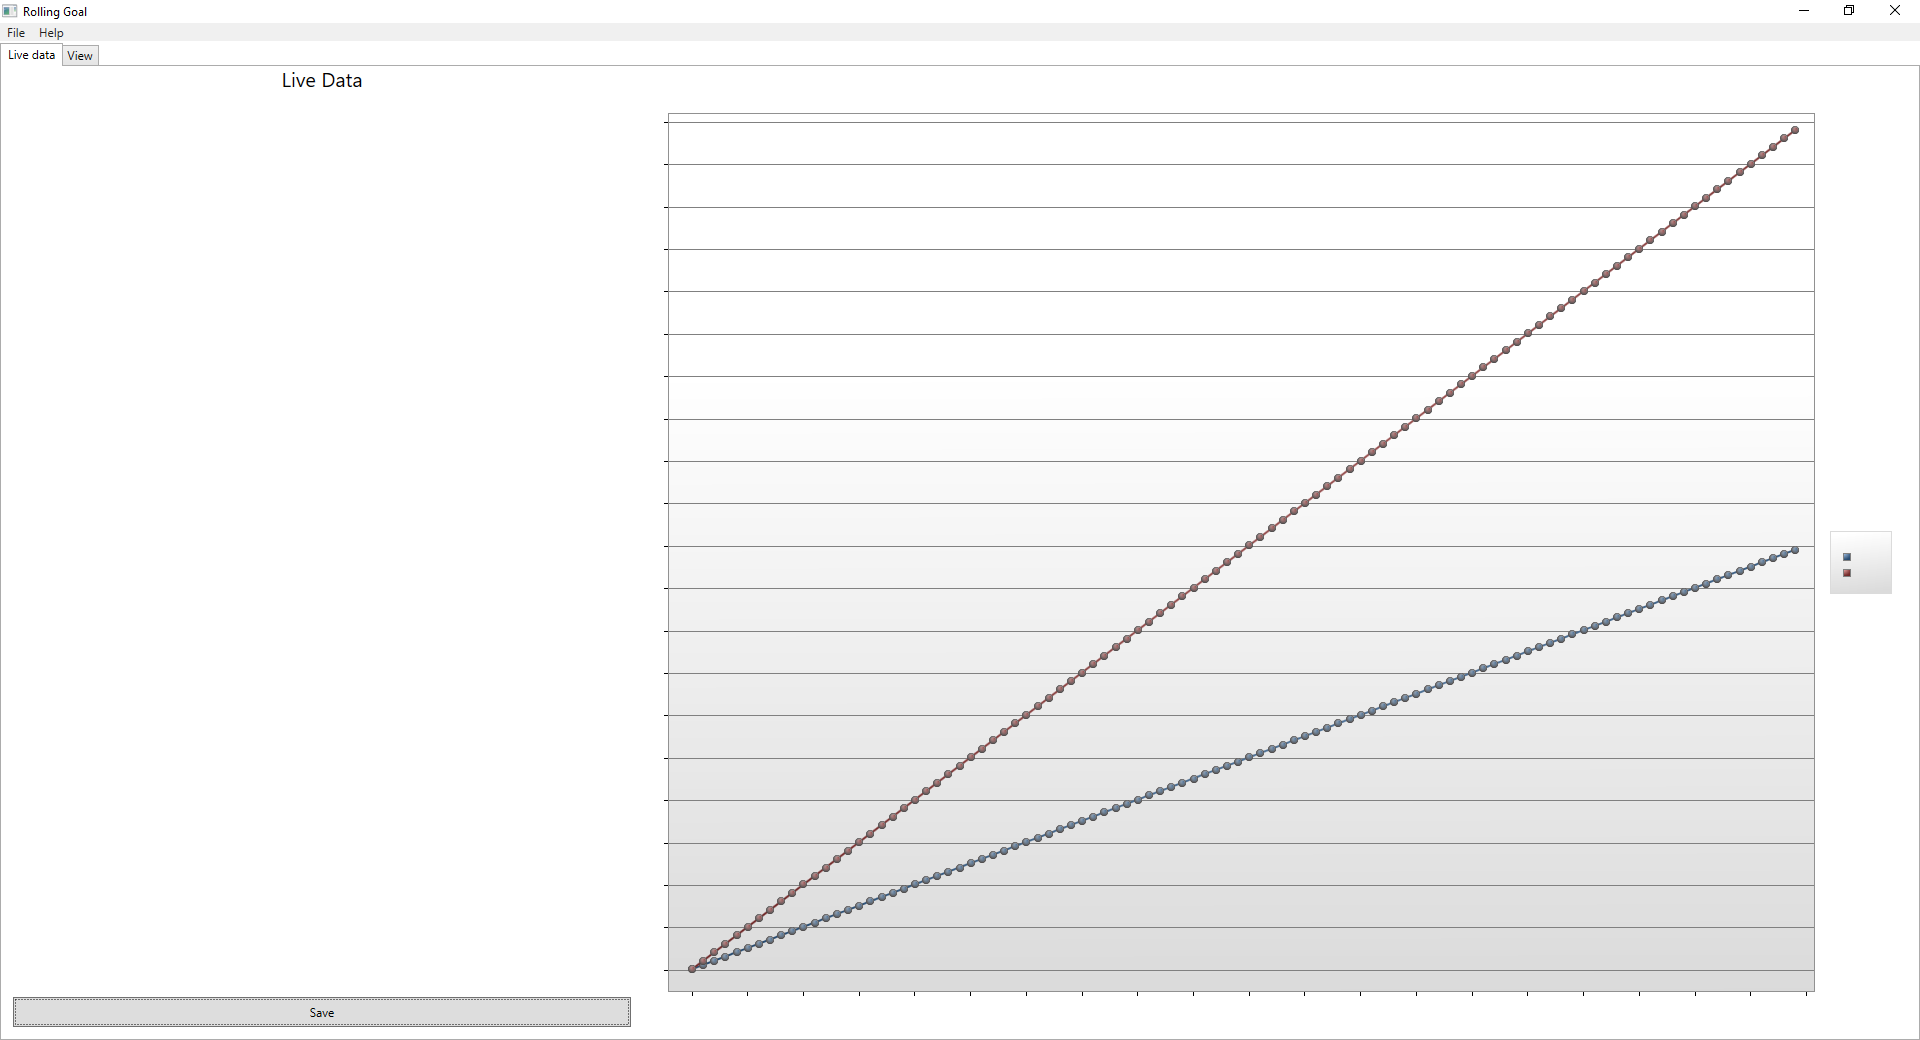
\includegraphics[width=0.7\linewidth]{SubPages/Images/First_GUI}
\caption{First working graph using the WPF-toolkit}
\label{fig:First_GUI}
\end{figure}

\begin{figure}[h!]
\centering
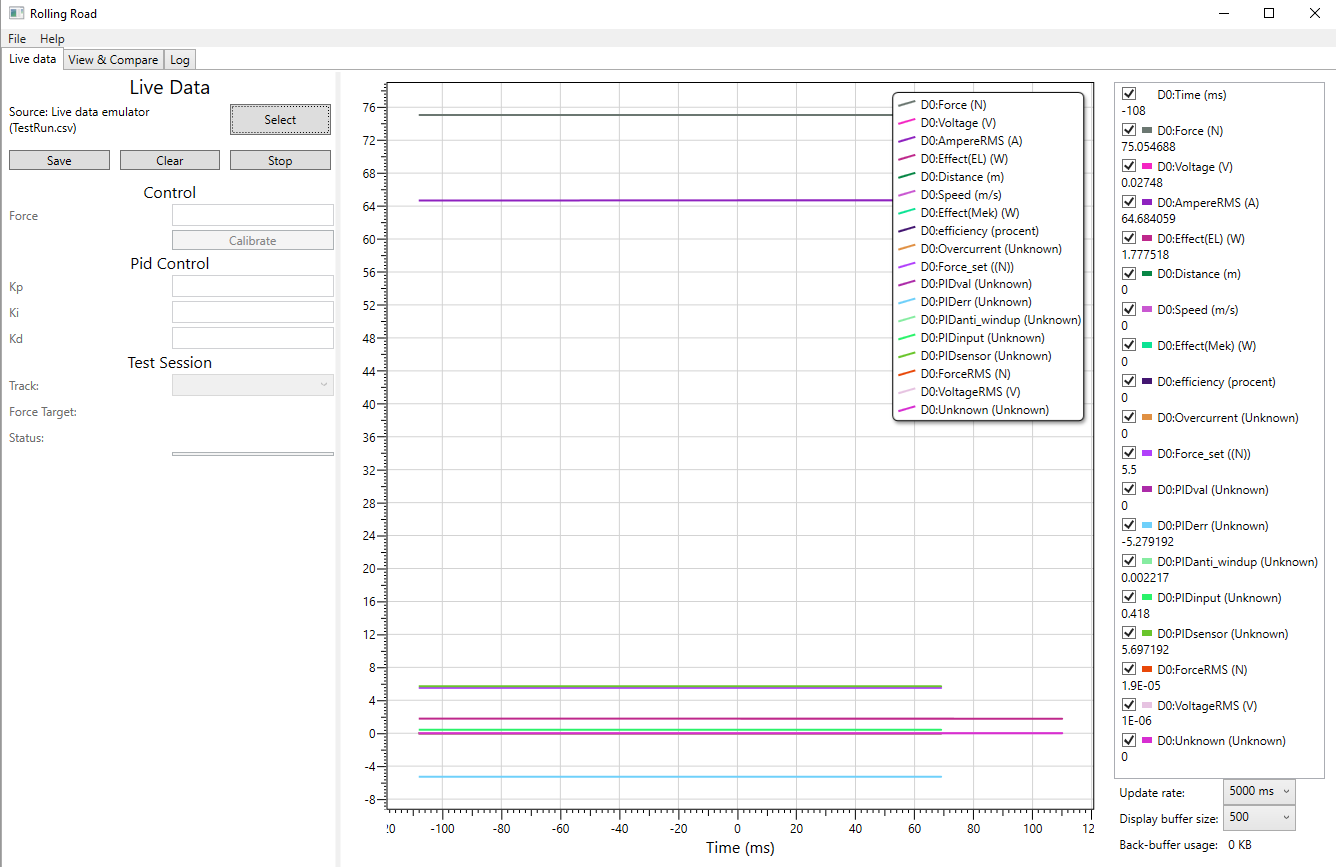
\includegraphics[width=0.7\linewidth]{SubPages/Images/Current_GUI}
\caption{Current GUI using the D3 library}
\label{fig:Current_GUI}
\end{figure}


\subsection{Testing}

For testing the GUI Application unit tests was written using the NUnit 3.* framework and NSubstitute as the Mock-framework to help isolate units under test.

This helped immensely when developing the SP4RR-interpreter, since it was developed before being able to integration test with the Rolling Road. It was done by mocking out the COM-Port stream and verifying the commands was sent and received as specified in SP4RR  protocol definition\cite{RR}.

\subsection{Continuous Integration}

From the start CI(Continuous Integration) was used to verify the code every time changes was detected in the repository. It was tested by running a series af code-tests and -analyzing tools, the steps used in the CI are as follows:

\begin{enumerate}
	\item Download all missing or out of date packages from Nuget
	\item Build the project
	\item Run all unit-tests
	\item Calculate code-coverage
	\item Duplicates finder
	\item Inspection
\end{enumerate}

Using CI also gives a history of the amount of test as seen in figure \vref{fig:CI_TestCount}

\begin{figure}[H]
\centering
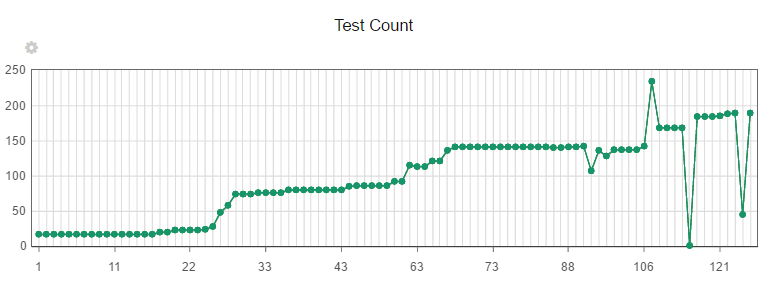
\includegraphics[width=0.95\linewidth]{SubPages/Images/CI_TestCount}
\caption{A plot of test count. Y-Axis: Test-count, X-Axis: Build number}
\label{fig:CI_TestCount}
\end{figure}
